% ---------------------------------------------------------------------------
% Author guideline and sample document for EG publication using LaTeX2e input
% D.Fellner, v1.14, Nov. 29, 2017

\documentclass{egpubl}
\usepackage{eurovis2018}

% --- for  Annual CONFERENCE
% \ConferenceSubmission   % uncomment for Conference submission
% \ConferencePaper        % uncomment for (final) Conference Paper
\STAR                   % uncomment for STAR contribution
% \Tutorial               % uncomment for Tutorial contribution
% \ShortPresentation      % uncomment for (final) Short Conference Presentation
% \Areas                  % uncomment for Areas contribution
% \MedicalPrize           % uncomment for Medical Prize contribution
% \Education              % uncomment for Education contribution
% \Poster                 % uncomment for Poster contribution
% \DC                     % uncomment for Doctoral Consortium
%
% --- for  CGF Journal
% \JournalSubmission    % uncomment for submission to Computer Graphics Forum
% \JournalPaper         % uncomment for final version of Journal Paper
%
% --- for  CGF Journal: special issue
% \SpecialIssueSubmission    % uncomment for submission to , special issue
% \SpecialIssuePaper         % uncomment for final version of Computer Graphics Forum, special issue
%                          % EuroVis, SGP, Rendering, PG
% --- for  EG Workshop Proceedings
% \WsSubmission      % uncomment for submission to EG Workshop
% \WsPaper           % uncomment for final version of EG Workshop contribution
% \WsSubmissionJoint % for joint events, for example ICAT-EGVE
% \WsPaperJoint      % for joint events, for example ICAT-EGVE
% \Expressive        % for SBIM, CAe, NPAR
% \DigitalHeritagePaper
% \PaperL2P          % for events EG only asks for License to Publish

% --- for EuroVis 
% for full papers use \SpecialIssuePaper
 \STAREurovis   % for EuroVis additional material 
% \EuroVisPoster % for EuroVis additional material 
% \EuroVisShort  % for EuroVis additional material

%
 \electronicVersion % can be used both for the printed and electronic version

% !! *please* don't change anything above
% !! unless you REALLY know what you are doing
% ------------------------------------------------------------------------

% for including postscript figures
% mind: package option 'draft' will replace PS figure by a filname within a frame
\ifpdf \usepackage[pdftex]{graphicx} \pdfcompresslevel=9
\else \usepackage[dvips]{graphicx} \fi

\PrintedOrElectronic

% prepare for electronic version of your document
\usepackage{t1enc,dfadobe}

\usepackage{egweblnk}
\usepackage{cite}

% For backwards compatibility to old LaTeX type font selection.
% Uncomment if your document adheres to LaTeX2e recommendations.
% \let\rm=\rmfamily    \let\sf=\sffamily    \let\tt=\ttfamily
% \let\it=\itshape     \let\sl=\slshape     \let\sc=\scshape
% \let\bf=\bfseries

% end of prologue


\usepackage[utf8]{inputenc}
\usepackage{xcolor}
\usepackage{tikz}
\usetikzlibrary{calc}
\usetikzlibrary{arrows.meta}
\usetikzlibrary{positioning}
\usepackage{amsmath}
\usepackage{amsfonts}
%\usepackage{todonotes}
\newcommand\todo[1]{\textit{\textcolor{blue}{\\TODO: #1\\}}}
\newcommand\todoi[1]{\textit{\textcolor{blue}{TODO: #1}}}
\newcommand\tcb[1]{\textit{\textcolor{blue}{#1}}}

\newcommand\bx[0]{\textbf{x}}
\newcommand\by[0]{\textbf{y}}
\newcommand\bomega[0]{\boldsymbol{\omega}}


\usepackage{import}
\usepackage{xifthen}
\usepackage{pdfpages}
\usepackage{transparent}
\newcommand{\incfig}[1]{%
    \def\svgwidth{\columnwidth}
    \import{./img/}{#1.pdf_tex}
}

% ---------------------------------------------------------------------
% EG author guidelines plus sample file for EG publication using LaTeX2e input
% D.Fellner, v2.02, Jan 25, 2017


\title[Participating Media]%
      {Rendering Participating Media}

% for anonymous conference submission please enter your SUBMISSION ID
% instead of the author's name (and leave the affiliation blank) !!
\author[B.Börcsök \& L.Leonard]
{\parbox{\textwidth}{\centering Barnabás Börcsök$^1$% 
\\ Seminar: Data Visualization %
\\ barnabas.borcsok@gmail.com% 
\\ Supervisor: Ludwig Leonard-Méndez^1%
%        S. Spencer$^2$\thanks{Chairman Siggraph Publications Board}
        }
        \\
% For Computer Graphics Forum: Please use the abbreviation of your first name.
{\parbox{\textwidth}{\centering $^1$ Technische Universit\"at M\"unchen
%        $^2$ Another Department to illustrate the use in papers from authors
%             with different affiliations
       }
}
}
% ------------------------------------------------------------------------

% if the Editors-in-Chief have given you the data, you may uncomment
% the following five lines and insert it here
%
% \volume{36}   % the volume in which the issue will be published;
% \issue{1}     % the issue number of the publication
% \pStartPage{1}      % set starting page


%-------------------------------------------------------------------------
\begin{document}

\teaser{ 
    
\includegraphics[width=\linewidth]{img/teaser.png}
    \centering
    \caption{Examples of participating media.}
    \label{fig:teaser}
}

\maketitle
%-------------------------------------------------------------------------
\begin{abstract}
    Rendering participating media such as smoke, fog, clouds and fire is 
    an important and active branch of computer graphics research. 
    This essay aims to give an overview of rendering such 
    volumetric phenomena by formalizing the problem statement, and building
    up to current advancements and directions of research in the field of
    rendering participating media.
   
%The tool at \url{http://dl.acm.org/ccs.cfm} can be used to generate
% CCS codes.
\begin{CCSXML}
<ccs2012>
   <concept>
       <concept_id>10010147.10010371.10010372</concept_id>
       <concept_desc>Computing methodologies~Rendering</concept_desc>
       <concept_significance>500</concept_significance>
       </concept>
 </ccs2012>
\end{CCSXML}

\ccsdesc[500]{Computing methodologies~Rendering}

\printccsdesc   
\end{abstract}  
%-------------------------------------------------------------------------
\section{Introduction}
%One of the aims of computer graphics is to reproduce the illusion of real life in a computer. In theory, a viewer should not be able to tell the difference between looking out on a window in real life, or looking at a computer scene. This noble (and seemingly unreachable) goal draws closer and closer to us each year with rapid developments in many fields of computer graphics. On one hand, we have to simulate events and phenomena happening around us, but we also have to put it on display in a manner that reproduces the look of real life as closely as possible. This is called rendering the virtual world. We will have a closer look at the latter, more specifically at techniques on how to render participating media.

Participating media affect the light as it tries to propagate through its volume. Some of the common examples include glass, water, smoke, and even clear air. (See Figure \ref{fig:teaser}.) We approach the rendering of such phenomena as a collection of particles interacting with light rays. Chapter \ref{section:properties-of-the-volume}
defines these possible interactions, laying the foundation for Chapter 
\ref{section:mathematical-foundations}
to formalize a possible extension of the widely used surface rendering 
equation, first introduced by \cite{Kaj86}. 

The main contribution of this paper is an overview of rendering participating media, building up the necessary formulations, and also giving a stable starting point for the interested reader to build up and understand more advanced techniques. 

This paper builds for the most parts on the 2017 SIGGRAPH course on \textit{Production
Volume Rendering} \cite{SG17} and on the 2018 survey on 
\textit{Monte Carlo Methods for Volumetric Light Transport Simulation} \cite{Novak18}.

As the use of ray tracing and Monte Carlo rendering is prevalent in current state-of-the-art production rendering engines \cite{SG17}, we also formalize the problem of rendering participating media as a ray-tracing problem, utilizing stochastic techniques to solve the equations.

The use of Monte Carlo techniques means that we model the interactions between particles and media as a probability field, modeling the "average effect" instead of the individual collision effects.

As photons, making up the light rays, propagate through participating media,
the ray's direction and radiance (ultimately perceived as color) changes.
This change in the light ray's direction and/or radiance is attributable
to collisions with particles assumed to be infinitesimal volumes, that make up
the whole of the participating media, as outlined in Section 
\ref{section:properties-of-the-volume}.
In essence, as these modified light rays end up reaching our eyes (or more 
precisely, our virtual camera), we end up seeing the phenomena at hand.

We assume \textit{statistically independent} collisions. This means that the 
methods discussed will work in any gaseous media (e.g. clouds, smoke, fog, 
fire, etc), but not for dense granular media such as sand and snow, where these assumptions break down.

The prerequisite for the above assumption is that the size of the particles should
be negligible compared to the average distance between them. If the particles are 
comparable to the average distance between them (which is the case for dense 
granular media), the assumption of statistically independent collisions breaks 
down, as a collision event results in a big deviation compared to a case where the
event does not happen.
%-------------------------------------------------------------------------
\section{Properties of the medium}
\label{section:properties-of-the-volume}
After a brief introduction to our goal and assumptions, we now dive deeper into how we think about participating media, and define important properties of the materials.

\subsection{Collision coefficients}
Participating media is a collection of microscopic particles.

As a photon travels through a medium (in the computer graphics sense), it interacts with material particles, which results in a loss of radiance due to the material absorbing the energy of the photon, or scattering it in some different directions. It is also possible for the photon particle to gain radiance due to the material's emission of energy, and also due to collecting the light scattered previously at some other point in the volume.

The \textit{absorption coefficient} $\sigma_a$ and 
\textit{scattering coefficient} $\sigma_s$ each quantify the local 
probability density of a photon undergoing the respective interaction per unit distance traveled $[\frac{1}{m}]$. For an overview of the possible interactions, see Figure \ref{fig:interactions}.

\begin{figure}[ht]
    \centering
    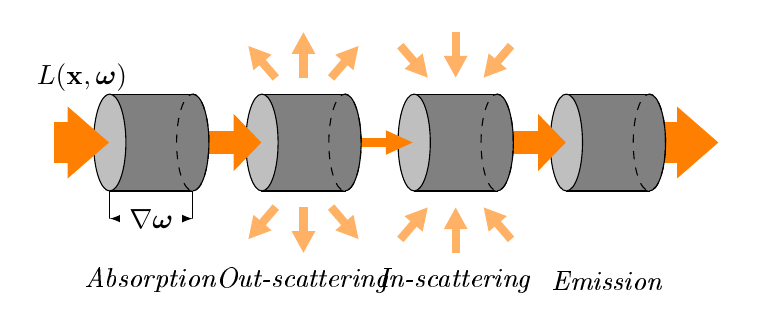
\begin{tikzpicture}
% 1 = 20p
    \def\XSTART{-10pt}
    \def\YSTART{60pt}
    \def\YDIAONE{35pt}
    \def\XONESTART{10pt}
    \def\XONEDELTA{30pt} %width of cylinders
    \def\DD{-10pt} %
    \def\GAP{25pt} %
    
    \def\LABELYSHIFT{-50pt}
    
    %FIRST cylinder
    \def\YEND{\YSTART+\YCURVE+\YDIATWO}
    \def\XONEEND{\XONESTART+\XONEDELTA}
    \def\YONEMIDDLE{\YSTART+\YDIAONE/2}
  
    %SECOND cylinder
    \def\XTWOSTART{\XONESTART+\XONEDELTA+\GAP}
    \def\XTWOEND{\XONEEND+\GAP+\XONEDELTA}
  
    %THIRD cylinder
    \def\XTHREESTART{\XONESTART+\XONEDELTA+\GAP+\XONEDELTA+\GAP}
    \def\XTHREEEND{\XONEEND+\GAP+\XONEDELTA+\GAP+\XONEDELTA}
    
    % FOURTH cylinder
    \def\XFOURSTART{\XONESTART+\XONEDELTA+\GAP+\XONEDELTA+\GAP+\XONEDELTA+\GAP}
    \def\XFOUREND{\XONEEND+\GAP+\XONEDELTA+\GAP+\XONEDELTA+\GAP+\XONEDELTA}

    \tikzset{
      partial ellipse/.style args={#1:#2:#3}{
          insert path={+ (#1:#3) arc (#1:#2:#3)}
      },
      dimen/.style={<->,>=latex,thin,
        every rectangle node/.style={fill=white,midway,font=\sffamily}},
    }
  
    % OUTGOING ARROW (EMISSION)
    \draw[-{Triangle[width=25pt,length=15pt, color=orange]}, 
            line width=15pt, color=orange]
        (\XFOUREND+0.5,\YONEMIDDLE) -- (\XFOUREND+\GAP,\YONEMIDDLE);

    %FOURTH CYLINDER
    \draw [fill=gray] (\XFOURSTART,\YSTART) coordinate (BA)
        rectangle (\XFOUREND,{\YSTART+\YDIAONE}) coordinate (BB);
    \draw [fill=lightgray](\XFOURSTART,\YONEMIDDLE)
        ellipse ({\YDIAONE/6} and {\YDIAONE/2});
    \draw [fill=gray,dashed](\XFOUREND,\YONEMIDDLE)
        ellipse ({\YDIAONE/6} and {\YDIAONE/2});
    \draw (\XFOUREND,\YONEMIDDLE)
        [partial ellipse=-90:90:{\YDIAONE/6} and {\YDIAONE/2}];

    \node[yshift=\LABELYSHIFT] at ($0.5*(BA)+0.5*(BB)$) {\textit{Emission}};

    % FIFTH ARROW (IN-SCATTERING)
    \draw[-{Triangle[width=20pt,length=10pt, color=orange]}, 
            line width=8pt, color=orange]
        (\XTHREEEND+0.5,\YONEMIDDLE) -- (\XTHREEEND+\GAP-0.2,\YONEMIDDLE);
    

    % INSCATTERING ARROWS AROUND THIRD CYLINDER
    % above
    \draw[-{Triangle[width=8pt,length=8pt, color=orange!60]}, 
            line width=3pt, color=orange!60]
        ({\XTHREESTART+\XONEDELTA/2},{\YONEMIDDLE+40pt}) --
        ({\XTHREESTART+\XONEDELTA/2},{\YONEMIDDLE+\YDIAONE/1.5});
    \draw[-{Triangle[width=8pt,length=8pt, color=orange!60]}, 
            line width=3pt, color=orange!60]
        ({\XTHREESTART+\XONEDELTA/2-20pt},{\YONEMIDDLE+35pt}) --
        ({\XTHREESTART+\XONEDELTA/2-10pt},{\YONEMIDDLE+\YDIAONE/1.5});
    \draw[-{Triangle[width=8pt,length=8pt, color=orange!60]}, 
            line width=3pt, color=orange!60]
        ({\XTHREESTART+\XONEDELTA/2+20pt},{\YONEMIDDLE+35pt}) --
        ({\XTHREESTART+\XONEDELTA/2+10pt},{\YONEMIDDLE+\YDIAONE/1.5});
    % below
    \draw[-{Triangle[width=8pt,length=8pt, color=orange!60]}, 
            line width=3pt, color=orange!60]
        ({\XTHREESTART+\XONEDELTA/2},{\YONEMIDDLE-40pt}) --
        ({\XTHREESTART+\XONEDELTA/2},{\YONEMIDDLE-\YDIAONE/1.5});
    \draw[-{Triangle[width=8pt,length=8pt, color=orange!60]}, 
            line width=3pt, color=orange!60]
        ({\XTHREESTART+\XONEDELTA/2-20pt},{\YONEMIDDLE-35pt}) -- 
        ({\XTHREESTART+\XONEDELTA/2-10pt},{\YONEMIDDLE-\YDIAONE/1.5});
    \draw[-{Triangle[width=8pt,length=8pt, color=orange!60]}, 
            line width=3pt, color=orange!60]
        ({\XTHREESTART+\XONEDELTA/2+20pt},{\YONEMIDDLE-35pt}) --
        ({\XTHREESTART+\XONEDELTA/2+10pt},{\YONEMIDDLE-\YDIAONE/1.5});

    \draw [fill=gray] (\XTHREESTART,\YSTART) coordinate (BA)
        rectangle (\XTHREEEND,{\YSTART+\YDIAONE}) coordinate (BB);
    \draw [fill=lightgray](\XTHREESTART,\YONEMIDDLE)
        ellipse ({\YDIAONE/6} and {\YDIAONE/2});
    \draw [fill=gray,dashed](\XTHREEEND,\YONEMIDDLE)
        ellipse ({\YDIAONE/6} and {\YDIAONE/2});
    \draw (\XTHREEEND,\YONEMIDDLE)
        [partial ellipse=-90:90:{\YDIAONE/6} and {\YDIAONE/2}];

    \node[yshift=\LABELYSHIFT] at ($0.5*(BA)+0.5*(BB)$) {\textit{In-scattering}};

    % THIRD ARROW (OUT-SCATTERING)
    \draw[-{Triangle[width=8pt,length=10pt, color=orange]}, 
            line width=3pt, color=orange]
        (\XTWOEND+0.5,\YONEMIDDLE) -- ({\XTWOEND+\GAP-0.2},\YONEMIDDLE);
    
        % OUTSCATTERING ARROWS AROUND SECOND CYLINDER
    % above
    \draw[-{Triangle[width=8pt,length=8pt, color=orange!60]}, 
            line width=3pt, color=orange!60]
        ({\XTWOSTART+\XONEDELTA/2},{\YONEMIDDLE+\YDIAONE/1.5}) -- 
        ({\XTWOSTART+\XONEDELTA/2},{\YONEMIDDLE+40pt});
    \draw[-{Triangle[width=8pt,length=8pt, color=orange!60]}, 
            line width=3pt, color=orange!60]
        ({\XTWOSTART+\XONEDELTA/2-10pt},{\YONEMIDDLE+\YDIAONE/1.5}) -- 
        ({\XTWOSTART+\XONEDELTA/2-20pt},{\YONEMIDDLE+35pt});
    \draw[-{Triangle[width=8pt,length=8pt, color=orange!60]}, 
            line width=3pt, color=orange!60]
        ({\XTWOSTART+\XONEDELTA/2+10pt},{\YONEMIDDLE+\YDIAONE/1.5}) -- 
        ({\XTWOSTART+\XONEDELTA/2+20pt},{\YONEMIDDLE+35pt});
    % below
    \draw[-{Triangle[width=8pt,length=8pt, color=orange!60]}, 
            line width=3pt, color=orange!60]
        ({\XTWOSTART+\XONEDELTA/2},{\YONEMIDDLE-\YDIAONE/1.5}) -- 
        ({\XTWOSTART+\XONEDELTA/2},{\YONEMIDDLE-40pt});
    \draw[-{Triangle[width=8pt,length=8pt, color=orange!60]}, 
            line width=3pt, color=orange!60]
        ({\XTWOSTART+\XONEDELTA/2-10pt},{\YONEMIDDLE-\YDIAONE/1.5}) -- 
        ({\XTWOSTART+\XONEDELTA/2-20pt},{\YONEMIDDLE-35pt});
    \draw[-{Triangle[width=8pt,length=8pt, color=orange!60]}, 
            line width=3pt, color=orange!60]
        ({\XTWOSTART+\XONEDELTA/2+10pt},{\YONEMIDDLE-\YDIAONE/1.5}) -- 
        ({\XTWOSTART+\XONEDELTA/2+20pt},{\YONEMIDDLE-35pt});

    % SECOND CYLINDER
    \draw [fill=gray] (\XTWOSTART,\YSTART) coordinate (BA)
        rectangle (\XTWOEND,{\YSTART+\YDIAONE}) coordinate (BB);
    \draw [fill=lightgray](\XTWOSTART,\YONEMIDDLE)
        ellipse ({\YDIAONE/6} and {\YDIAONE/2});
    \draw [fill=gray,dashed](\XTWOEND,\YONEMIDDLE)
        ellipse ({\YDIAONE/6} and {\YDIAONE/2});
    \draw (\XTWOEND,\YONEMIDDLE)
        [partial ellipse=-90:90:{\YDIAONE/6} and {\YDIAONE/2}];

    \node[yshift=\LABELYSHIFT] at ($0.5*(BA)+0.5*(BB)$) {\textit{Out-scattering}};
    
    % SECOND ARROW
    \draw[-{Triangle[width=20pt,length=10pt, color=orange]}, 
            line width=8pt, color=orange]
        ({\XONEEND+0.5},\YONEMIDDLE) -- ({\XONEEND+\GAP-0.2},\YONEMIDDLE);
    
    % FIRST CYLINDER
    \draw [fill=gray] (\XONESTART,\YSTART) coordinate (BA)
        rectangle (\XONEEND,{\YSTART+\YDIAONE}) coordinate (BB);
    \draw [fill=lightgray](\XONESTART,\YONEMIDDLE)
        ellipse ({\YDIAONE/6} and {\YDIAONE/2});
    \draw [fill=gray,dashed](\XONEEND,\YONEMIDDLE)
        ellipse ({\YDIAONE/6} and {\YDIAONE/2});
    \draw (\XONEEND,\YONEMIDDLE)
        [partial ellipse=-90:90:{\YDIAONE/6} and {\YDIAONE/2}];

    \node[yshift=\LABELYSHIFT] at ($0.5*(BA)+0.5*(BB)$) {\textit{Absorption}};
    
    %nabla omega below
    \draw ($(BB)-(0,\YDIAONE)$) -- ++(0,\DD) coordinate (D1) -- +(0,5pt);
    \draw (BA) -- ++(0,\DD) coordinate (D2) -- +(0,5pt);
    \draw [dimen] (D1) -- (D2) node {$\nabla\boldsymbol\omega$};

    % INCOMING ARROW
    \draw[-{Triangle[width=25pt,length=15pt, color=orange]}, 
            line width=15pt, color=orange]
            node [above=85pt ] {$\textcolor{black}{L(\textbf{x},\boldsymbol\omega)}$}
        (\XSTART,\YONEMIDDLE) -- (\XONESTART-0.2,\YONEMIDDLE);


    %ground
    %\draw [fill=gray] (0,0) rectangle  (\XEND,\GROUND);

\end{tikzpicture}%

    \caption{
        Possible interactions between the volume and the light traveling through the medium. In this example, it first loses $\sigma_a L(x, \omega)$ radiance due to the material absorbing a portion of the light, then loses further $\sigma_s L(x, \omega)$ due to out-scattering. Then it gains $\sigma_s L_i(x, \omega)$ radiance from light scattered at another part of the volume. Lastly, it gains $\sigma_a L_e(x, \omega)$ light due to the material's emission.
    }
    \label{fig:interactions}
\end{figure}

The \textit{extinction coefficient} $\sigma_t = \sigma_a + \sigma_s$ indicates
the probability density of either type of event happening per unit distance.
It is also called the \textit{attenuation coefficient}.

\subsection{Phase function}

The \textit{phase function} 
$f_p(\textbf{x}, \boldsymbol{\omega},\boldsymbol{\omega}')$
describes how the volume scatters light at a given point \bx, depending on the incident ($\bomega$) and outgoing ($\bomega'$) directions.

In order to influence only the direction of the light (but do not influence the intensity of the light), $f_p$ needs to be normalized over the unit sphere:
$
    \int f_p(\textbf{x}, \boldsymbol{\omega},\boldsymbol{\omega}') = 1.
$

Its use is analog to the BSDF function in the case of surface rendering. In most cases, $f_p$ can be written as a function of the single angle~$\theta$ between the two directions $\boldsymbol{\omega}$ and $\boldsymbol{\omega}'$. If the medium scatters light uniformly in all directions, it is said to be \textit{isotropic}, and the phase function is
$
    f_{p, isotropic}(\textbf{x}, \boldsymbol{\omega},\boldsymbol{\omega}') = 
    1/(4\pi).
$

\noindent If the phase function is not isotropic, then it is \textit{anisotropic}.


\subsection{Directional dependence}
In cases when the collision coefficients $\sigma_a$ and $\sigma_s$ do not depend on the direction of light propagation, the phase function can be parameterized only by the angle between incident and scattered light. A material is then called \textit{isotropic}. (Note: for isotropic materials, the phase function can still be anisotropic -- not scattering light uniformly.)

A material is \textit{anisotropic}, if the collision coefficients or the phase functions depend on the direction of incident or scattered light, i.e. the response of the material varies with the direction of propagation.

\subsection{Spatial dependence}
The medium is \textit{homogeneous} if all of the above medium properties are spatially invariant, and \textit{heterogeneous} otherwise.
%-------------------------------------------------------------------------
\section{Mathematical foundations for radiative transport}
\label{section:mathematical-foundations}
The physical phenomenon of radiative transport is the transfer of energy
in the form of electromagnetic radiation. In our case, we will deal with the transport of 
light, more precisely the interactions defining a photon traveling through participating media. For an overview of notation used, see Appendix \ref{appendix:notation}.

\subsection{Radiative Transfer Equation (RTE)}

The Radiative Transfer Equation (RTE) gives us the change in radiance traveling along direction $\omega$ through a differential volume element at point $\bx$. 
Appendix \ref{appendix:RTE} gives a detailed derivation of the RTE function, and its components before arriving at the \textit{integral form of the RTE}, giving us the explicit function

\begin{equation} \label{eq:RTE-int}
L(\bx, \bomega) = \int_0^\infty 
%T(\bx, \by)
e^{-\int_0^y{\sigma_t(\bx-s\bomega)}ds}
\Big[
    \sigma_s(\by)L_s(\by, \bomega) + \sigma_a(\by)L_e(\by, \bomega)
\Big]
d\by,
\end{equation}

which is suitable for use in a path tracing setting.
We call $e^{-\int_0^y{\sigma_t(\bx-t\bomega)}}$ the  
\textit{transmittance coefficient} and denote it with $T(\bx, \by)$,
summing up the loss of light intensity between $\bx$ and 
$\by$ due to absorption and out-scattering by integrating a single differential 
process along $\bomega$. The exponent
$\int_0^y{\sigma_t(\bx-s\bomega)}$ 
is called the \textit{optical thickness} $\tau$. This is the Beer-Lambert law \cite{Lambert}, and we will often simplify the notation of the
function to take only a single parameter $t$, denoting the distance between $\bx$ and
$\textbf{y}$: $T(t) = e^{-\tau(t)} =e^{-\int_0^t{\mu_t(\boldsymbol{x}-s\boldsymbol\omega)}ds}$.

\subsection{Volume rendering equation}
As scenes are usually not made up only of participating media, but also solid objects
with hard boundaries, we have to extend Equation~(\ref{eq:RTE-int}) to also 
accommodate light interactions with object surfaces. The radiative equilibrium at a surface point $\textbf{z}$ is given by the surface rendering equation \cite{Kaj86}:

\begin{equation}\label{eq:surface}
    L(\textbf{z}, \bomega) = L_e(\textbf{z}, \bomega) +
    \int_{S^2} f_r(\textbf{z},\bomega,\bomega')L_i(\textbf{z},\bomega')
    ~\big| n(\textbf{z}\cdot \bomega')\big|~ d \omega' ,
\end{equation}

\noindent where $L_e(\textbf{z}, \bomega)$ is the radiance emitted by the surface, $f_r(\textbf{z},\bomega,\bomega')$ is the BSDF (Bidirectional Scattering Function), relating the differential outgoing radiance $dL(\textbf{z},\bomega)$ to the incident radiance $L_i(\textbf{z}, \bomega')$,
and $\big| n(\textbf{z}\cdot \bomega')\big|$ is a foreshortening term depending on the surface normal $n(\textbf{z},\bomega')$ at incident point $\textbf{z}$ and incident ray direction $\bomega'$.

We can combine Equations (\ref{eq:RTE-int}) and (\ref{eq:surface}) into the Volume Rendering Equation (VRE):

\begin{align}
\begin{aligned}
\label{eq:VRE}
L(\bx, \bomega) = &\int_{0}^{z} 
    T(\bx, \by)
    \big[ 
        \sigma_a(\by)L_e(\by, \bomega) + 
        \sigma_s(\by)L_s(\by, \bomega)
    \big] dy
    \\ + 
    &T(\bx, \textbf{z})L(\textbf{z},\bomega).
\end{aligned}
\end{align}

Given a closest surface point $\textbf{z}$, our volumetric rendering equation holds true up until this point, giving us the boundary condition for truncating the bounds of Equation~(\ref{eq:RTE-int}). (As we have to calculate the propagation of the light ray in the media up until this point.) 
The radiance at this point $\textbf{z}$ is given by Equation~(\ref{eq:surface}) in direction $\bomega$. 
$L(\textbf{z}, \bomega)$ represents the exitant radiance from the surface given by Equation~(\ref{eq:surface}), and the fraction of this that actually reaches our point $\bx$ is given by the transmittance coefficient $T(\bx, \by)$. 

\begin{figure}[ht]
    \centering
    \incfig{vre}
    \caption{The Volume Rendering Equation (VRE) visualized.}
    \label{fig:vre}
\end{figure}

\subsection{Monte Carlo integration}
Practically all modern high-quality physically-based rendering engines use Monte Carlo integration to solve the aforementioned equations.

A \textit{primary} Monte Carlo estimator $\langle F \rangle = f(x) / p(x)$ is used to approximate $F(x)$'s integrand $f(x)$, where the probability density function (PDF) $p(x)$ is used to sample points $x$. Averaging $N$ independent realizations of a primary estimator, one can obtain a \textit{secondary} (i.e. multi-sample) estimator. 

We can use a Monte Carlo estimator to solve the Volume Rendering Equation (\ref{eq:VRE}), estimating the amount of radiance arriving at point $\bx$ from direction $\bomega$:

\begin{align}
\begin{aligned}
\label{eq:MC-VRE}
\langle L(\bx, \bomega) \rangle 
=&
    \frac{T(\bx, \by)}{p(y)}
    \big[ 
        \sigma_a(\by)L_e(\by, \bomega) + 
        \sigma_s(\by)L_s(\by, \bomega)
    \big]
    \\ +& 
    T(\bx, \textbf{z}) L(\textbf{z},\bomega),
\end{aligned}
\end{align}

\noindent where $p(y)$ is the PDF of sampling point $\by$, which is $y$ units away from $\bx$. This estimator requires two main routines: one for sampling distances along the ray, and one for estimating the transmittance $T(\bx, \by)$ between two given points. We will discuss these in Section \ref{section:distance-sampling} and \ref{section:transmittance} respectively.

Estimator \ref{eq:MC-VRE} gives us a somewhat \textit{localized} view on the light-transport simulation, as we consider only one path segment at a time. For a more \textit{global} view on the transport problem, one can also utilize the path integral framework\cite{MLT-1}, enabling the sampling of entire sequence of vertices at once, in contrast to (\ref{eq:MC-VRE}) sampling only one vertex at once. Examples of such global techniques are joint importance sampling\cite{joint-importance} and Metropolis sampling \cite{MLT-2}. As we will not discuss these techniques here, the interested reader might want to refer to the cited sources.

Whatever the sampling technique might be, two fundamental building blocks should be considered. Firstly, sampling a distance in a given direction, which is covered in Section \ref{section:distance-sampling}. This is used, as we construct our ray, propagating from the sensor (or virtual camera) into our virtual scene (and most notably, into the participating media). On the other hand, some techniques do not perform analog walks by sampling distances, but instead rely on estimating the transmittance between two points. We will cover transmittance estimation in Section \ref{section:transmittance}.

%-------------------------------------------------------------------------
\section{Distance sampling}
\label{section:distance-sampling}
In this and the next section, we discuss techniques for sampling distances and estimating transmittance along a ray. To classify distance-sampling methods, we share the terminology of \textit{analog} and \textit{non-analog} estimators of \cite{Novak18}, which they borrowed from the field of neutron transport. They categorize the algorithms according to whether they strictly adhere to the physical process of light propagation (analog), or not (non-analog).

\textit{Analog} methods sample the distance to the next light-medium collision along the line of flight analogously to how photons interact with materials in the real world. The sampling procedure is in such cases commonly referred to as \textit{free-path sampling} or \textit{free-flight-distance sampling}. The distance distribution strictly adheres to the Beer-Lambert law: it has a PDF proportional to the transmittance along the given ray. Sampling can be explicit, via inverting the corresponding cumulative distribution function (CDF), or implicit, through probabilistic reasoning as in null-collision algorithms (discussed in \ref{section:delta}).

\textit{Non-analog} methods have been developed to improve sampling efficiency over analog methods. They deviate from the true distribution of free paths, which are then "corrected" by appropriately weighting the samples. They usually lift some restriction present in analog methods. As we will not concentrate on these non-analog techniques, the interested reader may refer to \cite{Novak18}.

Distance sampling is essential in the common case where a path is constructed incrementally by successively extending it from the sensor to the lights. 

Methods share the common theme of sampling distances according to a certain probability density function (PDF). In the following, we first review analytic and semi-analytic analog methods for media that allows free-path sampling in closed form or through a simple iterative process. Next, we discuss rejection-based analog estimators that rely on so-called \textit{null collisions}. 

\subsection{Closed-form tracking in homogeneous volume}

For sampling purposes, we can define a PDF by normalizing the transmittance function $T(t) = \text{e}^{-\int_{s=0}^t \sigma_t (\bx_s)ds}$. 

If the corresponding Cumulative Distribution Function (CDF) is analytically invertible, then the free-path distance $t'$ can be sampled analytically using a single random number $\zeta$.

For the homogeneous volume, where $\sigma_t$ is not spatially varying, the transmittance becomes
$$
T(t) = e^{-\sigma_t t},
$$
which is the Beer-Lambert law: exponential extinction of radiance. We would like a free-flight estimator, that produces a free-path distance $t'$, the distance a proton will travel in the volume. The PDF to do so is defined by normalizing the integral of the exponential function of the transmittance:
$
p(t) = \sigma_t e^{-\sigma_t t}.
$

\noindent We can perfectly importance sample the PDF (producing a weight of 1) with the analytic formula for sampling free paths using uniform random numbers $\zeta \in [0,1)$,\cite{PharrHumphrey2016}:
$
t' = - ln(1 - \zeta)/\sigma_t,   
$
with PDF 
\begin{equation}\label{eq:mc-pdf}
p(t) = \sigma_t e^{-\sigma_t t}.
\end{equation}

\subsection{Regular tracking}
In piecewise constant volumes, we can apply closed-form tracking to each of the piecewise constant domains, simply traversing into the next domain if we do not scatter. We can interpret the surface radiance $L(\textbf{z}, \bomega)$ as coming not from a hit surface, but rather a different volume. Finding boundaries separating homogeneous areas can introduce a substantial computing overhead. In order to be efficient, this approach needs large parts of the volume to be homogeneous. 

\subsubsection{Ray marching}
We can reduce the cost of regular tracking, by ignoring the boundaries and marching along the ray with fixed-size steps. This significantly simplifies the implementation at the cost of introducing bias. The algorithm queries the local medium extinction and then moves forward by a fixed distance. We assume either constant or linear optical thickness between the sampling points, deviating from the true free-path distribution. Sampling more frequently is always an option, although this adds to the computational costs. One way to reduce the cost can be to locally adapt the step size, or introduce other more sophisticated methods, such as higher order ray marching schemes\cite{Munoz14}. 

\subsection{Delta tracking}\label{section:delta}
Also known as Woodcock tracking, the null-collision algorithm, or pseudo scattering, the main idea behind delta tracking dates back to the rejection sampling technique introduced by John von Neumann in 1951\cite{vonNeumann1951}.

The key idea to sampling free-path distances is to homogenize the collision density in heterogeneous volumes by introducing a fictitious collision type. By making the total collision density constant, the volume can be now considered homogeneous. In this new type of collision, called \textit{null-collision}, the volume scatters in the same direction as the incoming direction, having no effect on the light transport itself. We express this collision type with the null-collision coefficient $\sigma_n(\bx)$ which acts in the same way as the other physical coefficients introduced earlier. The physical collision coefficients are now spatially variant, as is the null-collision coefficient $\sigma_n(\bx)$. To homogenize the overall volume, we choose $\sigma_n(\bx)$ in such a way that the sum of all coefficients, the \textit{free-path coefficient $\bar{\sigma}$}, becomes constant:

\begin{equation}
\bar{\sigma} = \sigma_a(\bx) + \sigma_s(\bx) + \sigma_n(\bx) = \sigma_t(\bx) + \sigma_n(\bx).    
\end{equation}

\noindent A consequence of this is that $\bar\sigma$ is always equal or greater to the maximum of $\sigma_t(\bx)$, which is often formulated as being a \textit{majorant} of $\sigma_t(\bx)$:
$
    \bar{\sigma} \geq \sigma_t(\bx).
$

\noindent We can easily calculate $\sigma_n(\bx)$:
\begin{equation}
    \sigma_n(\bx) = \bar\sigma - \sigma_t(\bx).
\end{equation}

\noindent As $\bar\sigma$ is constant, it can take on the role of the constant extinction $\sigma_t$ used in the closed-form technique \ref{eq:mc-pdf} and we can draw a distance sample in the same way as in the closed-form tracking:
\begin{equation}\label{eq:mc-pn}
    p_n(t) = \bar{\sigma}~e^{-\bar\sigma t}.
\end{equation}

By introducing null-collisions, we now have three collision types instead of two, resulting in the definition of three probabilities to consider:
$$
P_a(\bx) = \frac{\sigma_a(\bx)}{\bar\sigma},~~~ 
P_s(\bx) = \frac{\sigma_s(\bx)}{\bar\sigma},~~~
P_n(\bx) = \frac{\sigma_n(\bx)}{\bar\sigma},
$$

\noindent where $P_a(\bx) + P_s(\bx) + P_n(\bx) = 1$. Applying the additional null-collision probability to the VRE gives the recursive form

\begin{align}
\begin{aligned}
    L(\bx_j, \omega_j) = \int_{t=0}^\infty 
    p_n(t_j)\Big[
        &P_a(\bx) L_e(\bx_{j+1}, \omega_j) +\\
        &P_s(\bx) L_s(\bx_{j+1}, \omega_j) +\\
        &P_n(\bx) L(\bx_{j+1}, \omega_j)
    \Big]dt.
\end{aligned}
\end{align}

To work efficiently, we need $\bar\sigma$ to be as close to the maximum of $\sigma_t$ as possible. While it is valid, to just simply choose a very large $\bar\sigma$, that would result in having mostly null-collisions, stopping only to do nothing, and continue further.

%Introducing a null-collision type of (fictitious) volume-photon interaction, that does nothing to the photon when the interaction happens. We choose the null-collision coefficient $\sigma_n(\bx)$ such that the sampling strategy as used in closed form tracking sees a homogeneous (constant) volume.


%-------------------------------------------------------------------------
\section{Transmittance estimation}
\label{section:transmittance}
Transmittance $T(\bx, \by)$ gives us how likely it is for a photon to pass through the volume between points $\bx$ and $\by$ without undergoing absorption or out-scattering. This is also called \textit{free-flight estimation}. As mentioned before, the transmittance function can be simplified to taking in a single real value $t$, denoting the distance between $\bx$ and
$\by$.

Transmittance can be calculated by essentially marching along the ray (instead of using the Monte Carlo technique) accumulating the loss of light (e.g. transmittance). This however introduces bias, and also might result in rendering artifacts if the volume is undersampled. In production, a ray marching transmittance with very small step sizes can be used as a reference to validate more sophisticated implementations\cite{SG17}.

\subsection{Delta tracking transmittance estimator}
We can use Equation (\ref{eq:mc-pn}) as a transmittance estimator in the PDF approach, testing if a collision occured before or after distance $t$. This estimator produces a binary estimator: $T(t) = 1$ or $T(t) = 0$. This technique is \textit{unbiased}.\cite{Novak18} The mean of the samples is the transmittance, although the variance is large. This binary estimate might be considered to be too inaccurate to be used efficiently in the PDF approach as it either totally discards or lets through.\cite{SG17} However, the concept of adding null collisions opens up the possibility for other methods, that we describe in this section. 

\subsection{Ratio tracking transmittance estimator}
Introduced to computer graphics by \cite{novak2014residual}, the goal of ratio tracking methods is the same: estimating the percentage of photons that make it beyond distance $t$. The main idea is to remove the binary fashion of the estimation mentioned above, and instead weighting the samples by the probability of continuing the walk. 

In contrast to the aforementioned binary estimation, ratio tracking allows every single distance sample to reach $t$, scoring a fractional weight. The tracking \textit{never} terminates before $t$, and weight the accumulated transmittance at potential collision position $\textbf{c}$ by $\sigma_n(\textbf{c})/\bar\sigma(\textbf{c}) = 1- \sigma_t(\textbf{c})/\bar\sigma(\textbf{c})$, the "probability" of continuing forward. This can be formulated in the final transmittance estimator

\begin{equation}
    T(d) = \prod_{i=1}^K (1 - \frac{\sigma_t(\bx_i)}{\bar\sigma}),
\end{equation}

where $K$ are all of the collisions created before reaching the end of integration $d$. Like in delta tracking, the free path coefficient $\bar\sigma$ needs to be constant and a majorant of $\sigma_t(\bx_i)$.

An incremental improvement, called residual ratio tracking is also introduced by \cite{novak2014residual}. Refer to \ref{appendix:residual-ratio-tracking} for more details.
%-------------------------------------------------------------------------
\section{Acceleration Data Structures / Optimization}
Acceleration data structures are important, as \textit{data access} usually dominates the overall render time.

While ray tracing, an improvement can be achieved by \textit{avoiding empty spaces} before the first interaction with the volumetric effect.

In the case of delta tracking, having a \textit{localized $\bar\sigma$ majorant} for spatially diverse transmittance also yields performance gains, as we reduce the number of null collisions, which means we "stop, and continue without doing anything" fewer times. Space partitioning data structures, such as \textit{k-d trees}\cite{yue2010unbiased} or \textit{octrees}\cite{kutz2017spectral} might be used to achieve this.


%-------------------------------------------------------------------------
\section{Remaining challenges and open problems}
\subsection{Machine Learning}
As is the case with many others fields of computer graphics (and beyond), enhancing volumetric rendering with Artificial Intelligence (AI) methods, such as machine learning has huge potentials. The vast cost involved when accessing voxelized data and tracing paths in high-albedo volumes involving lots of scattering (e.g. clouds) make it challenging for Monte Carlo techniques to deliver results at tractable costs. The high expense of importance sampling such high-dimensional spaces can be mitigated by incorporating various aggregators \cite{AIaggr01}\cite{AIaggr02}\cite{AIaggr03}, diffusion approximations \cite{AIdiff01}\cite{AIdiff02}\cite{AIdiff03}\cite{AIdiff04} or deep learning \cite{AIdl}, but this always comes at the cost of introducing some kind of bias.
AI techniques can also be applied at the level of distance and directional samples for surface rendering \cite{AIsurf01}\cite{AIsurf02}\cite{AIsurf03}\cite{AIsurf04}, or other forms of path guiding could potentially provide significant benefits.

\subsection{Joint handling of surfaces and volumes}
A final render usually necessitates including both volumes and surfaces in the same scene. Different techniques have been developed to tackle these different tasks, which could even mean the usage of different renderers for surfaces and volumes in the same scenes, potentially leading to problems when combined. A unified scene representation might lend itself better for many use cases.


%-------------------------------------------------------------------------
\section{Conclusion}
In this seminar paper, we introduced the problem statement of rendering participating media. We formalized the problem in a way that is applicable to usual ray tracing methods utilized in rendering algorithms. We also looked at subtasks needed, namely distance sampling and transmittance estimation. Without going into more advanced techniques, our aim was to lay the foundations for further reading into the topic, and gave pointers to notable research papers.
%-------------------------------------------------------------------------

%\bibliographystyle{eg-alpha}
\bibliographystyle{eg-alpha-doi}

\bibliography{egbibsample}

\appendix

\section{Notation}\label{appendix:notation}
\begin{table}[h]
\centering
\begin{tabular}{|c|l|}
    \hline
    $\textbf{x, y}\in \mathbb{R}^3$ & 
    positions in 3D space \\
    $s \in \mathbb{R}$ &
    scalar value \\
    $\boldsymbol\omega \in \mathbb{R}^3$ & direction vector \\
    $\textbf{y} = \textbf{x}-s\boldsymbol\omega$ &
    $\textbf{y}$ is $s$ away from $\textbf{x}$ in direction $-\boldsymbol{\omega}$\\
    \hline
    $\textbf{x}_s := \textbf{x}-s\boldsymbol\omega$ &
    optional shorthands for the above\\
    $\textbf{x}_t := \textbf{x}-t\boldsymbol\omega$ & \\
    \hline
    $\by = \bx - y\bomega$ &
    $y$ denotes the distance of $\by$ from $\bx$.\\
    \hline
\end{tabular}
\caption{A quick overview of notation used}
\end{table}

Some papers denote the absorption, scattering and extinction coefficients
with $\mu_a$, $\mu_s$ and $\mu_e$ respectively, devising them
from the cross-sectional areas $[m^2]$ $\sigma_a$, $\sigma_s$ and $\sigma_t$
for absorbing, scattering and extinguishing (both absorbing \textit{and} scattering) 
particles and also the density per unit volume $\rho$ $[\frac{1}{m^3}]$.

They denote the above mentioned collision coefficients with 
$\mu_{a,s,t} = \sigma_{a,s,t}\cdot\rho$, multiplying the cross-sectional areas by 
the density per unity volume.

For the purposes of this seminar paper, we use the notations
introduced in Section \ref{section:mathematical-foundations}, denoting the absorption, scattering and extinction 
coefficients with $\sigma_{a}$, $\sigma_{s}$ and $\sigma_{t}$ respectively.

\section{Radiative Transfer Equation}\label{appendix:RTE}
The Radiative Transfer Equation (RTE) gives the change in radiance traveling along direction
$\bomega$ through a differential volume element at point $\textbf{x}$.

As a photon travels through a medium, it interacts with material particles, which
results in a loss of radiance due to absorption, and scattering in different directions 
\textit{(specified by the phase function $f_p$)}, while also gaining radiance due to the 
material's emission of energy, and collecting the scattered light from all directions.

We call the radiance loss due to the light scattering in all directions \textit{out-scattering}, and the radiance gain due to collecting the light scattered elsewhere \textit{in-scattering}.

We lose a portion of radiance $L(\bx, \bomega)$ due to absorption and out-scattering: $\sigma_a(\bx)L(\bx,\bomega)$ and $\sigma_s(\bx)L(\bx,\bomega)$, respectively. For brevity, we usually combine these into a single extinction term: $$\sigma_t(\bx)L(\bx, \bomega).$$

For calculating the \textit{radiance gains due to in-scattering}, we collect all incident radiance $L_i(\bx, \bomega)$ from all directions on the unit sphere $S^2$, and call it \textit{in-scattered radiance}:

$$L_s(\bx, \bomega) = \int_{S^2} f_p(\bomega, \bomega') L_i(\bx, \bomega') d\bomega'.$$ 

After calculating the in-scattered radiance, we multiply it with the $\sigma_s$ scattering coefficient, as light gets scattered in the direction of the viewer only if there are scattering particles there.

We can also gain radiance due to the volume emitting energy. The volume's emitted radiance is expressed as a radiance field $L_e(\bx, \bomega)$, whose output gets absorbed and scattered just like any other "regular", non-volume light source. If a volume does not emit, $L_e(\bx, \bomega)$ is simply zero.

Adding together these four terms, we arrive at the Radiative Transfer Equation (RTE):

\begin{align} 
\begin{aligned}
\label{eq:RTE}
(\bomega \nabla)L(\bx,\bomega) =&
- \sigma_t(\bx)L(\bx,\bomega) +\\
&+ \sigma_s(\bx)L_s(\bx,\bomega) + \sigma_a(\bx)L_e(\bx,\bomega).
\end{aligned}
\end{align}


Note: $(\bomega \nabla)$ is a notation for looking at the change in radiance L in direction $\bomega$.

Equation (\ref{eq:RTE}) gives us the change in radiance in a forward-transport fashion using the gradient $\bomega\nabla$, defining what happens to a radiance beam as it travels forward in direction $\bomega$, as can be seen on Figure \ref{fig:interactions}. This is useful for many applications, but not in a path tracing setting. Integrating Equation \ref{eq:RTE} along the direction $\bomega$, changing the gradient $(\bomega\nabla)$ on the left side into an integral on the right side, we arrive at the integral form of the Radiative Transfer Equation, giving us the explicit function

\begin{equation}
L(\bx, \bomega) = \int_0^\infty 
%T(\bx, \by)
e^{-\int_0^y{\sigma_t(\bx-s\bomega)}ds}
\Big[
    \sigma_s(\by)L_s(\by, \bomega) + \sigma_a(\by)L_e(\by, \bomega)
\Big]
d\by.
\end{equation}


\section{Residual ratio tracking}\label{appendix:residual-ratio-tracking}
Next to ratio tracking, \cite{novak2014residual} also introduced a more sophisticated technique called residual ratio tracking. It is an incremental improvement, introducing a control extinction coefficient $\sigma_c$, which is constant over the volume, and ideally is very similar to the actual extinction coefficient $\sigma_t$. With $\sigma_c$, the transmittance $T(t)$ is now broken into two parts: a control transmittance $T_c(t)$, which can be written in closed form, and a residual transmittance $T_r(t)$, which must be estimated:
\begin{align}
\begin{aligned}
    T_c(t) &= e^{-\sigma_c t}\\
    T_r(t) &= e^{-\int^t_{s=0} \sigma_t(\bx_s)-\sigma_c ds }\\
    T(t)   &= T_c(t) T_r(t)
\end{aligned}
\end{align}

The key improvement of residual ratio tracking  over ratio tracking is the use of $\bar\sigma_r$, the majorant over the residual extinction coefficient $\sigma_r = \sigma_t - \sigma_c$. 

\end{document}
